\documentclass[border=10pt]{standalone}

\usepackage{tikz}
\usepackage{tikzsymbols}
\usetikzlibrary{calc,patterns,shapes.geometric}

\def\centerarc[#1](#2)(#3:#4:#5){\draw[#1] ($(#2)+({#5*cos(#3)},{#5*sin(#3)})$) arc (#3:#4:#5);}

\begin{document}
	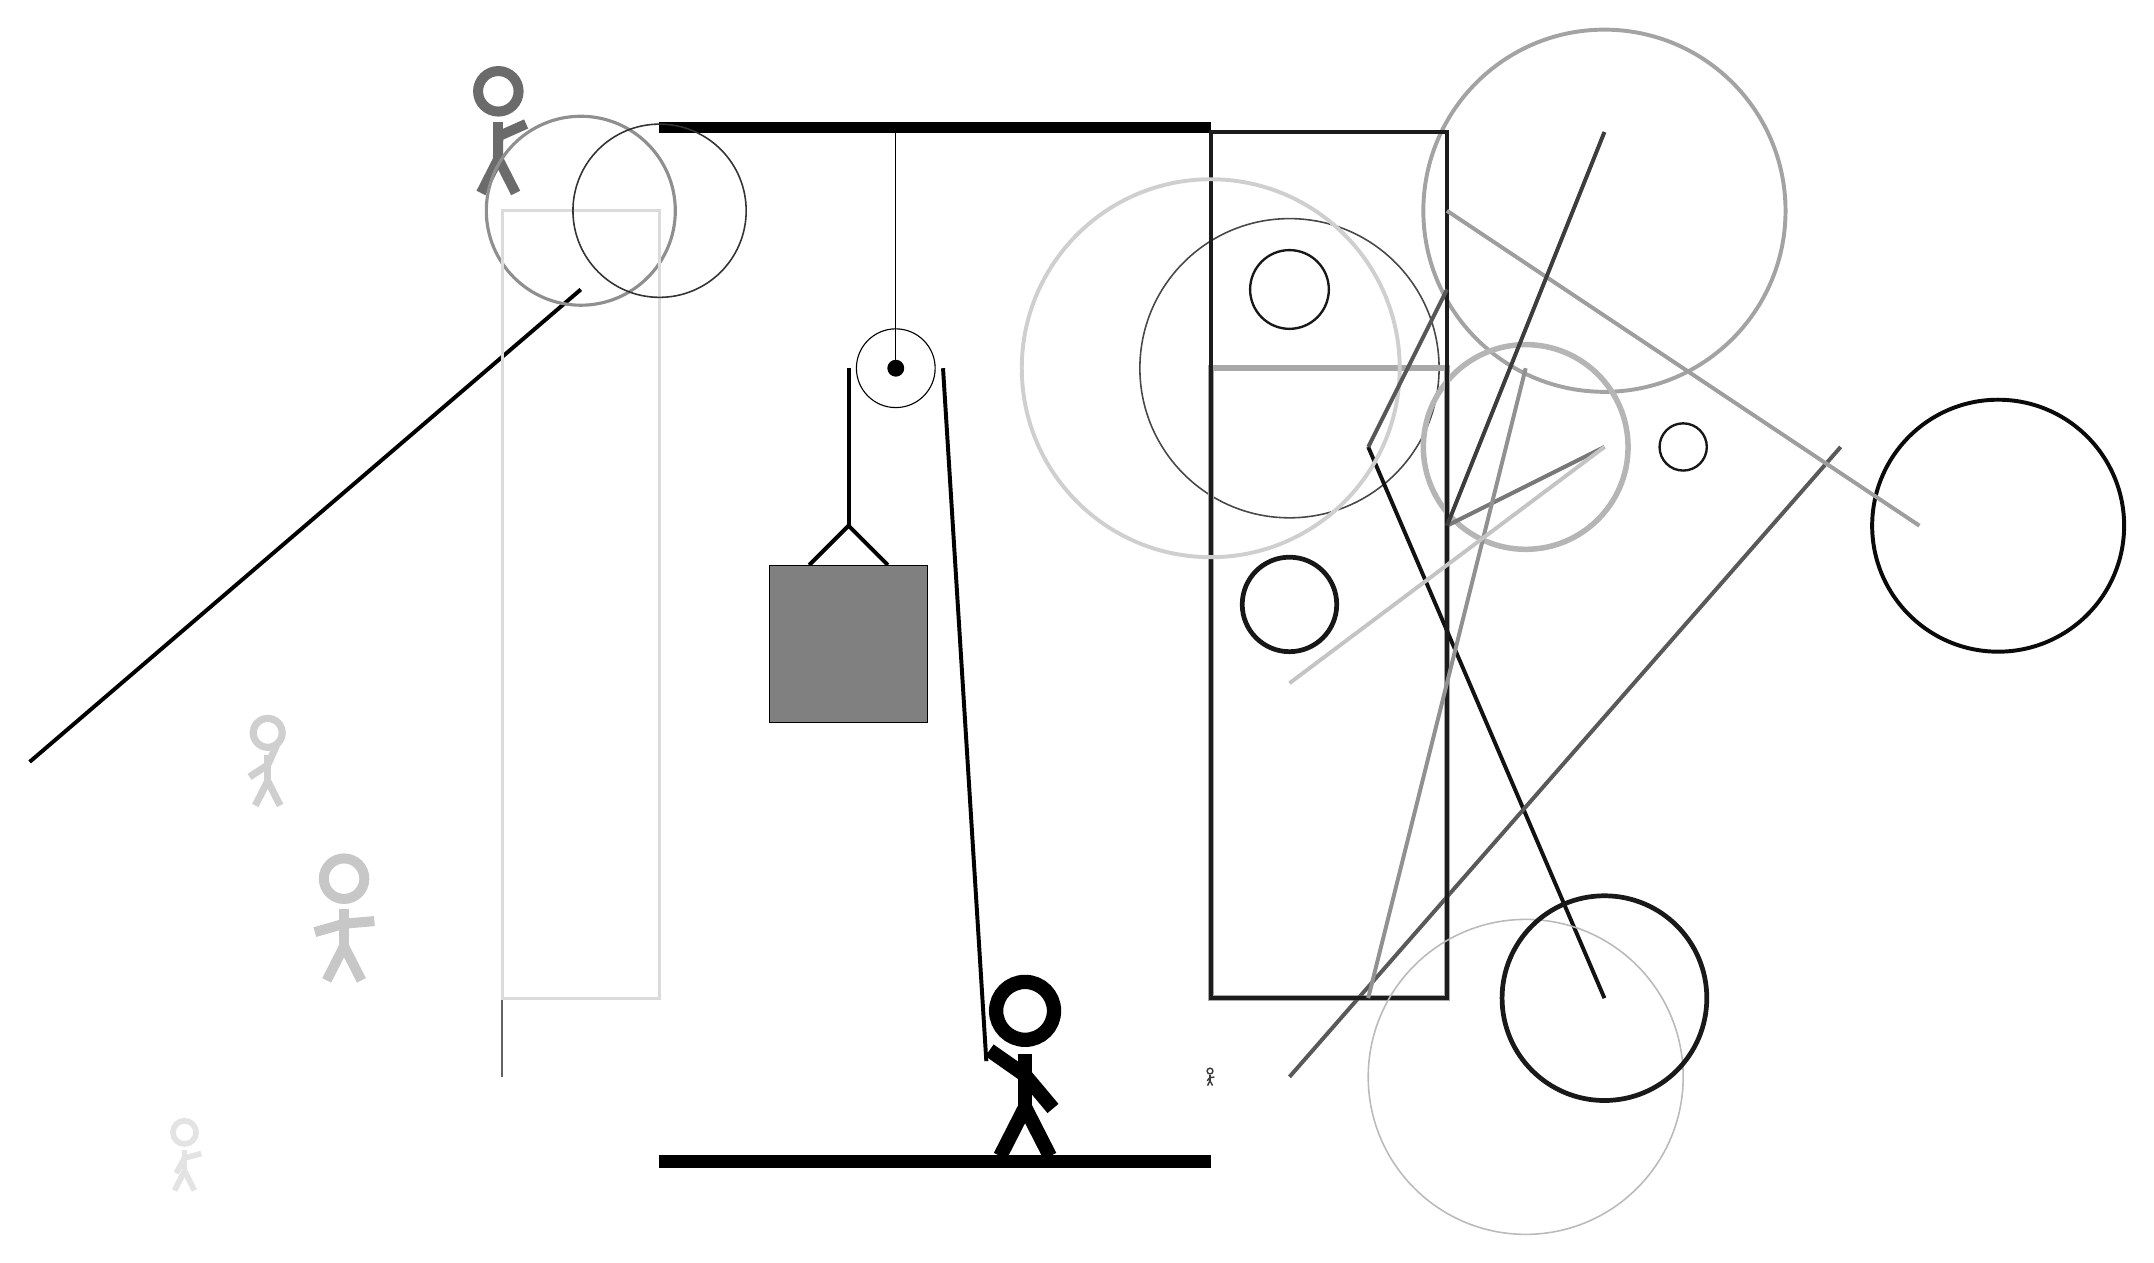
\begin{tikzpicture}
		%%%%% START %%%%%
		
		\draw[fill=black] (-2, 10) rectangle (5, 10.125);
		
		\draw (1, 7) circle (0.5);
		\draw[fill=black] (1, 7) circle (0.1);
		\draw (1, 10) -- (1, 7);
		
		\draw[line width=0.5mm] (-0.1, 4.5) -- (0.4, 5.0) -- (0.9, 4.5);
		\draw[fill=black!50] (-0.6, 4.5) rectangle (1.4, 2.5);
		
		\draw[line width=0.5mm] (0.4, 7) -- (0.4, 5.0);
		\centerarc[line width=0.5mm](1, 7)(0:180:0.6);
		\draw[line width=0.5mm](1.6, 7) -- (2.15, -1.8);
		
		\node at (2.6, -1.9) {\Strichmaxerl[10][-35][-50]};
		
		\draw [line width=0.3mm, color=black!91](11, 6) circle (0.3);
		
		\draw [line width=0.2mm, color=black!72](6, 7) circle (1.9);
		\draw[line width=0.7mm, color=black!34] (5, 7) rectangle (8, -1);
		\node[line width=0.4mm, color=black!77] at (5, -2) {\Strichmaxerl[1][48][5]};
		\draw [line width=0.5mm, color=black!36](10, 9) circle (2.3);
		\node[line width=0.4mm, color=black!58] at (-4, 10) {\Strichmaxerl[7][89][24]};
		\draw [line width=0.5mm, color=black!96](15, 5) circle (1.6);
		\draw [line width=0.7mm, color=black!29](9, 6) circle (1.3);
		\draw[line width=0.5mm, color=black!93](7, 6) -- (10, -1);
		\draw[line width=0.5mm, color=black!65](6, -2) -- (13, 6);
		\node[line width=0.7mm, color=black!11] at (-8, -3) {\Strichmaxerl[4][61][15]};
		\draw[line width=0.5mm, color=black!100](-3, 8) -- (-10, 2);
		\draw[line width=0.5mm, color=black!71](8, 2) -- (8, -1);
		
		\draw[line width=0.3mm, color=black!61] (-4, -2) rectangle (-4, 2);
		\draw[line width=0.5mm, color=black!53](10, 6) -- (8, 5);
		\draw[line width=0.5mm, color=black!89] (5, 10) rectangle (8, -1);
		\draw[line width=0.5mm, color=black!43](7, -1) -- (9, 7);
		\draw [line width=0.5mm, color=black!19](5, 7) circle (2.4);
		\draw [line width=0.4mm, color=black!44](-3, 9) circle (1.2);
		\draw[line width=0.5mm, color=black!38](8, 9) -- (14, 5);
		\draw [line width=0.6mm, color=black!91](6, 4) circle (0.6);
		
		\draw[line width=0.5mm, color=black!66](8, 8) -- (7, 6);
		\node[line width=0.3mm, color=black!19] at (-7, 2) {\Strichmaxerl[5][33][66]};
		\draw [line width=0.2mm, color=black!27](9, -2) circle (2.0);
		\draw[line width=0.4mm, color=black!14] (-4, -1) rectangle (-2, 9);
		
		\draw [line width=0.6mm, color=black!90](10, -1) circle (1.3);
		\draw [line width=0.2mm, color=black!80](-2, 9) circle (1.1);
		\draw[line width=0.5mm, color=black!76](10, 10) -- (8, 5);
		\draw [line width=0.3mm, color=black!91](6, 8) circle (0.5);
		\draw[line width=0.5mm, color=black!23](10, 6) -- (6, 3);
		\node[line width=0.5mm, color=black!22] at (-6, 0) {\Strichmaxerl[7][16][5]};
		
		
		\draw[fill=black] (-2, -3) rectangle (5, -3.15);
		
		%%%%% END %%%%%
	\end{tikzpicture}
\end{document}